\scanpage{19}
% L1–6. Continuation of the bracket opened on scan 18.
$\mathrm{Inf}$ d'une partie de $\unsure{P|\mathcal P|\Phi}$ (dans $P$) est $\varnothing$, i.e. si son
intersection ne contient pas d'él. de $P\setminus\{\varnothing\}$,
que cette intersection soit vide. Ex : \deleted{\unsure{un}} quadrilatère
qui n'est pas un parallélogramme
\figure{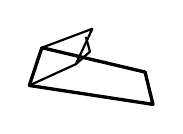
\begin{tikzpicture}[x=1cm,y=1cm,line cap=round,line join=round]
\draw[very thick] (0,0)--(.16,.48)--(1.47,.17)--(1.57,-.24)--cycle;
\draw[thick] (0,0)--(.59,.27)--(.8,.72)--(.16,.48);
\draw[thick] (.59,.27)--(.77,.43)--(.72,.61);
\end{tikzpicture}}.
L'axiome qui suit assure qu'il en est
pourtant ainsi\ldots{} ]

% L7–11
e) Si $b,b'$ sont des él. maximaux de $P$
\inserted{(i.e. $b,b'\in B$)} dont le $\inf$ est $\varnothing$ (i.e. $b'=\sigma b$), alors \deleted{\illegible{2}}
$b\cap b'=\varnothing$ (i.e., \deleted{\unsure{b,b'}} par d), \inserted{$b,b'$ sont \unsure{des|alors}}
\deleted{\unsure{2 à} des sous-variétés lin. parallèles}
hyperplans affines parallèles\ldots).

% L12–17
Dans l'espace des translations $T$ de $V$,
les \deleted{\unsure{des}} espaces directeurs $H_i$ $(i\in I)$ des
\deleted{\unsure{des}} deux \deleted{sous-espaces linéaires} \inserted{hyperplans affines} $b\in B$ sont
lin. indép, et correspondent donc à
une décomposition $\displaystyle T\simeq\prod T_i$ $(T_i=T/H_i)$
de $T$ en produit de droites. La donnée
% L18–24
du $T$-torseur $E$ revient à la donnée
d'une famille $(\deleted{T}E_i)_{i\in I}$ de $\deleted{\unsure{E}}T_i$-torseurs.
$E_i\simeq E/H_i$. De plus, dans chaque
$E_i$ il y a \inserted{une partie de} deux pts distincts, \deleted{\unsure{soit}} \unsure{q} $B_i$,
(isom. à la fibre de $B/I$ en $i\in I$). Or
on vérifie que la donnée \deleted{d'un} (pour $i$
% archive sheet number: 18
